\section{Hintergrund und verwandte Arbeiten}
\label{sec:Hintergrund und verwandte Arbeiten}

Dieses Kapitel gibt einen Überblick über die bestehenden Systeme zur Interaktion mit digitalen Zeichnungsumgebungen im Kontext der Raumplanung sowie über die technischen Grundlagen der entwickelten Lösung. Ziel ist es, die Relevanz des Projekts im bestehenden Lösungsraum aufzuzeigen und die Besonderheiten des eigenen Ansatzes zu motivieren. Zunächst wird der institutionelle Rahmen (SCDH) beschrieben, bevor im Anschluss technische Grundlagen, verwandte Systeme und der eigene Lösungsansatz vorgestellt werden.



\subsection{Projektkontext: Das SCDH und die bestehende Infrastruktur}

Das Projekt „The Architect's 1:1 Sandbox“ ist am Swiss Center for Design and Health (SCDH) in Nidau angesiedelt. Das SCDH betreibt eine Forschungsinfrastruktur, die es ermöglicht, Gebäudekonzepte im Massstab 1:1 mittels Projektoren und Mockups zu visualisieren. Diese Umgebung erlaubt es, architektonische Entwürfe gemeinsam mit Fachpersonen und Laien realitätsnah zu evaluieren und zu diskutieren.

Die Projektionsfläche des SCDH wird bislang primär verwendet, um bestehende Grundrisspläne darzustellen und physisch zu begehen. Interaktive Anpassungen oder kollaborative Zeichenvorgänge sind derzeit nur über analoge Mittel wie Papier oder Klebeband möglich. Die Integration einer digitalen Interaktionslösung stellt daher einen logischen nächsten Schritt zur Weiterentwicklung dieser Umgebung dar.

\begin{figure}[H]
    \centering
    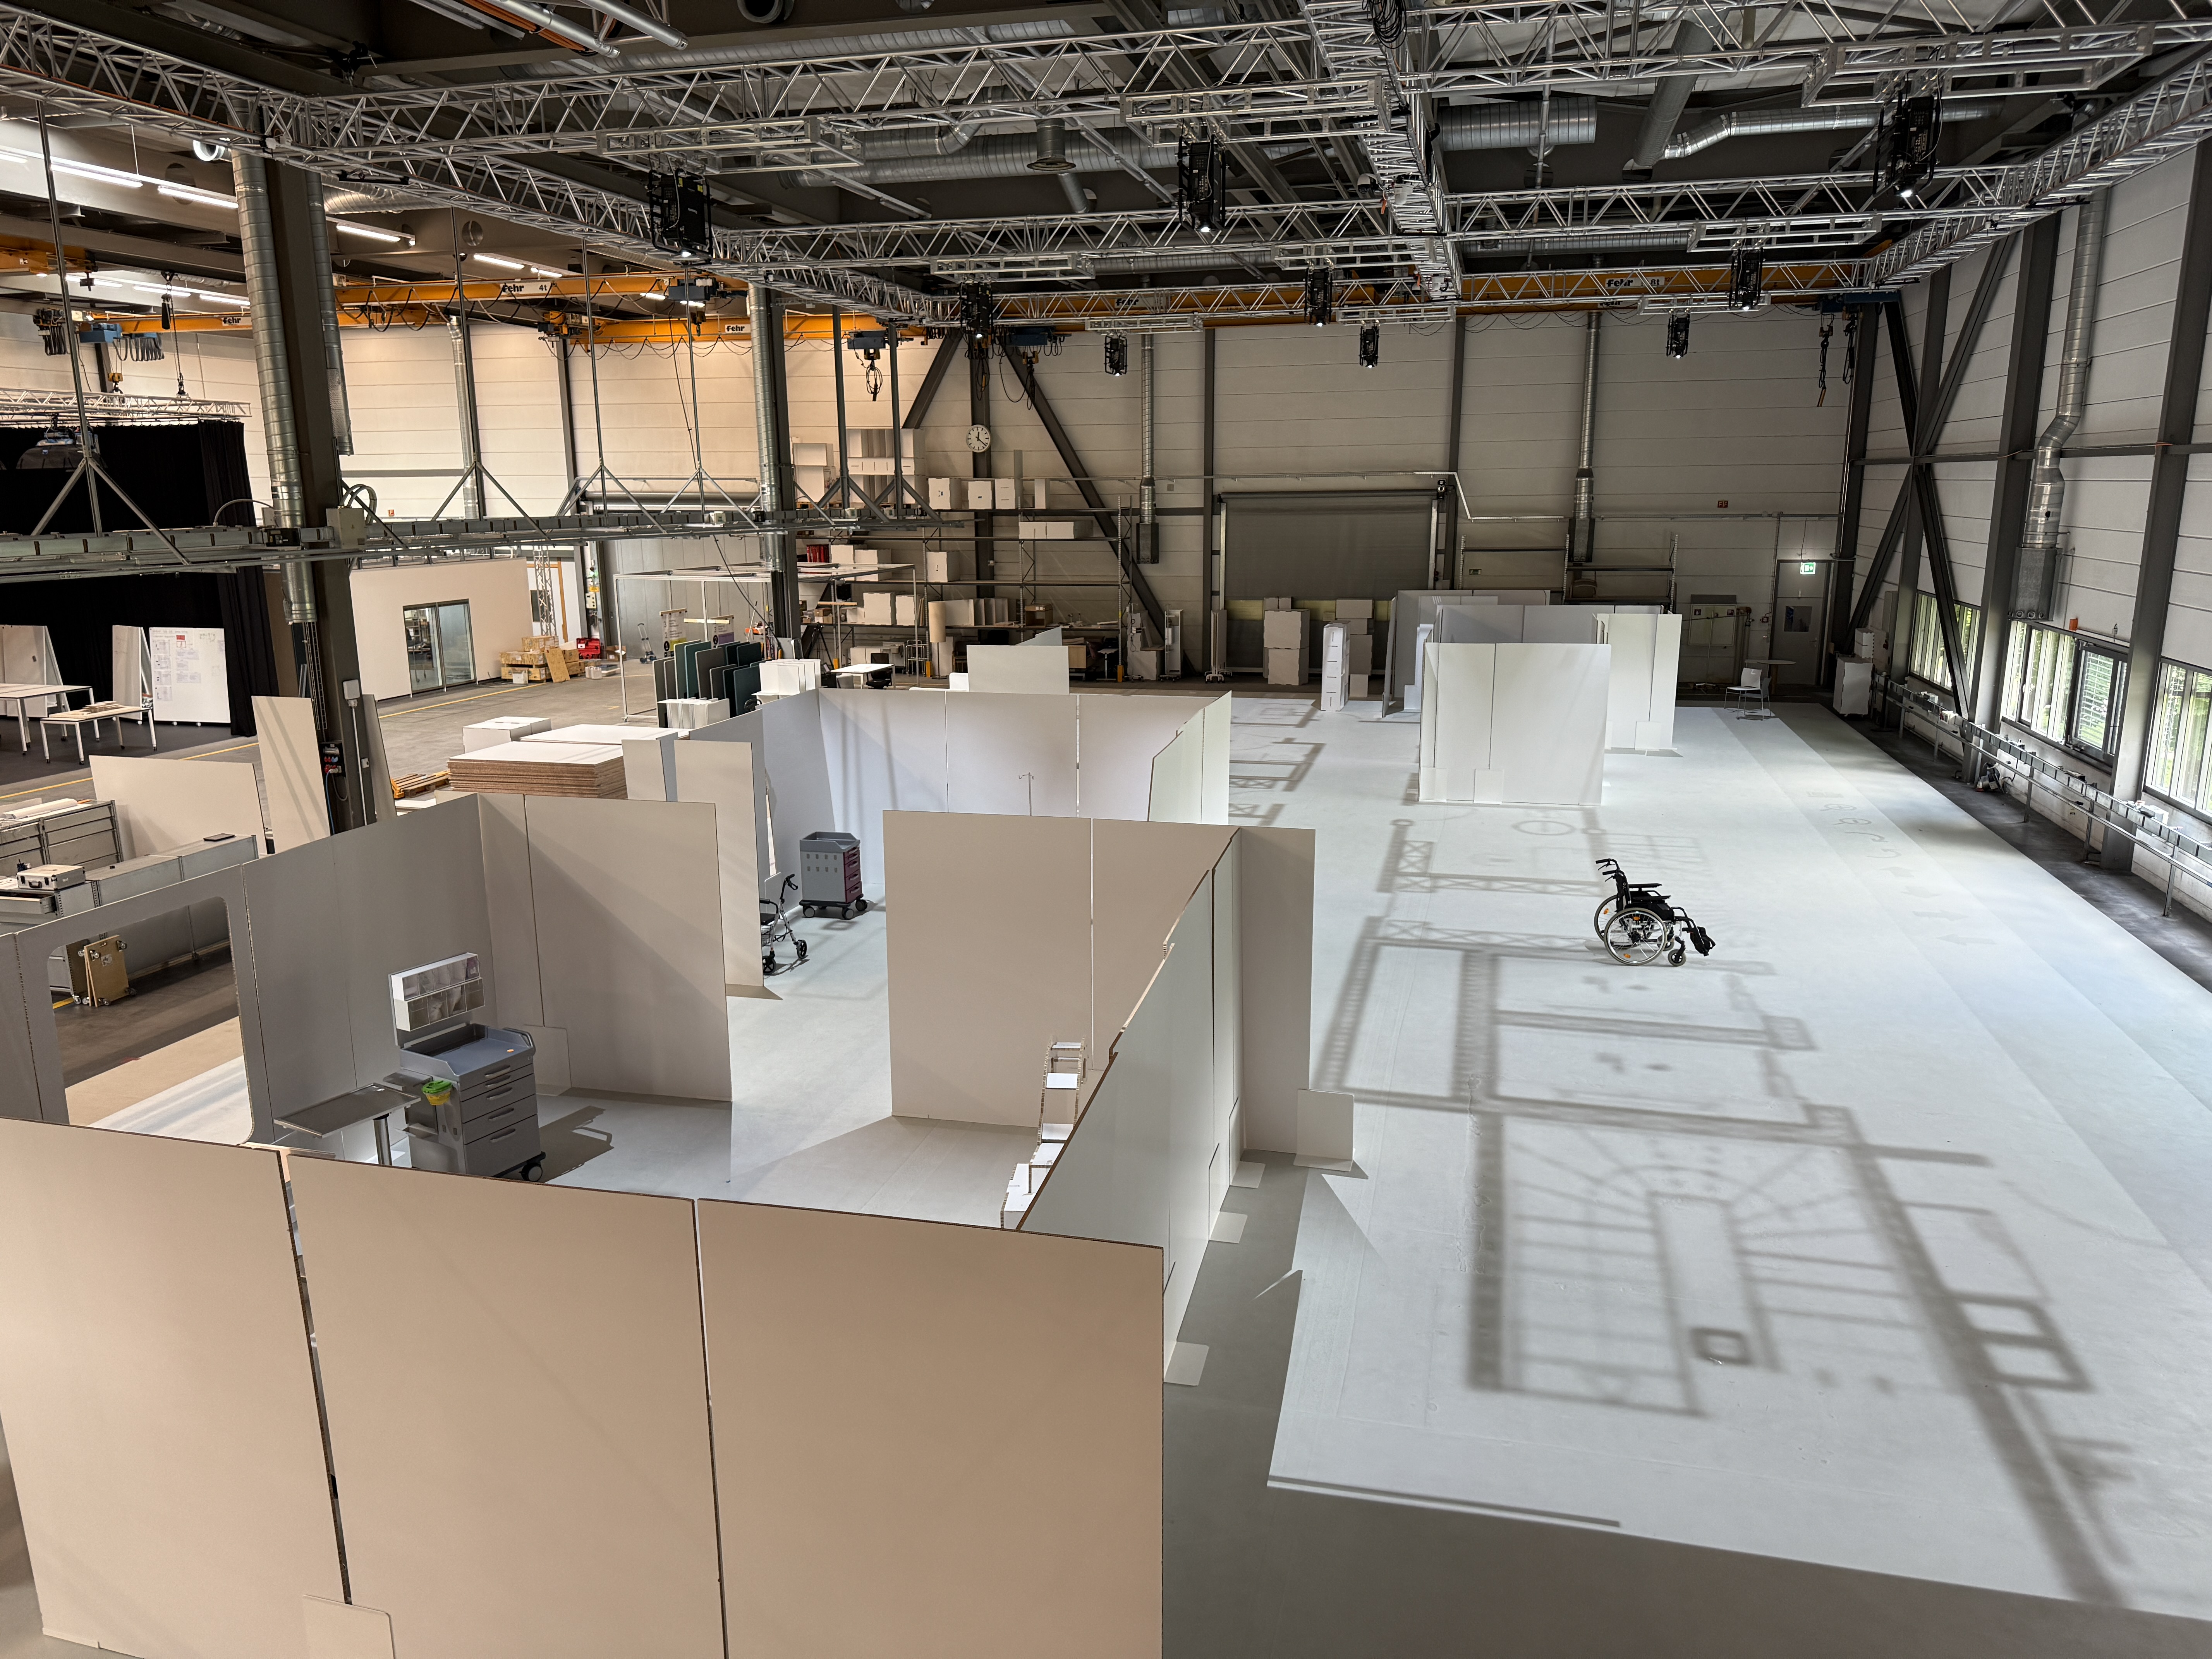
\includegraphics[width=0.75\linewidth]{graphics/Bild_vorhandene_infrastruktur.JPG}
    \caption{Bestehende Anlage mit Mockup}
    \label{fig:placeholder}
\end{figure}

\clearpage

\subsection{Technologische Grundlagen}

Die Umsetzung basiert auf einem Infrarotstift, der eine punktuelle IR-Lichtquelle erzeugt, welche von einer externen Infrarotkamera (Intel RealSense D455) erfasst wird, in einem Outside-in-Tracking-Verfahren. Durch Segmentierung und Schwellenwertverfahren werden die hellsten Bildbereiche isoliert, um die Position der Stiftspitze zu bestimmen.

Mithilfe einer sogenannten Homographie-Matrix wird der erkannte Punkt aus dem Kamerakoordinatensystem in die Zeichenfläche transformiert. Dies ermöglicht eine präzise Interaktion auf einer beliebigen, zuvor kalibrierten Projektionsfläche. Die Kalibrierung erfolgt durch das gezielte Ansteuern vordefinierter Referenzpunkte, aus denen die Projektionsgeometrie berechnet wird.

Die gesamte Lösung ist so konzipiert, dass sie plattformunabhängig (Windows, macOS, Linux) funktioniert und sich flexibel an unterschiedliche Projektionssituationen anpassen lässt.

\subsubsection{Inside-out and Outside-in tracking}

\textbf{Inside-out:}
Beim Inside-out Tracking befindet sich die Sensorik, die für die Positionsbestimmung des Stiftes notwendig ist, direkt am Stift (oder dem Gerät, das den Stift trackt). Der Stift ''sieht'' von innen nach aussen in seine Umgebung und nutzt dort vorhandene Merkmale (z.B. optische Marker, natürliche Landmarken oder Inertialsensoren) zur Bestimmung seiner eigenen Position und Orientierung im Raum.\\
\cite{tracking_source}

\textbf{Outside-in:}
Beim Outside-in Tracking ist die Sensorik extern und fest in der Umgebung des Stiftes platziert (z.B. Kameras, Basisstationen). Diese externen Sensoren ''beobachten'' den Stift (oder Marker/Signale am Stift) von aussen und bestimmen dessen Position und Orientierung im Raum.\\
\cite{tracking_source}
\subsubsection{Infrarot}

Bei Infrarotstrahlung handelt es sich um einen Bereich des elektromagnetischen Spektrums direkt unterhalb des sichtbaren roten Lichts. Der Infrarotbereich umfasst Wellenlängen von etwa 780\,nm bis 1\,mm. Dieser Spektralbereich ist für das menschliche Auge unsichtbar. Für das vorliegende Projekt ist der sogenannte nahe Infrarotbereich von 780\,nm bis 3000\,nm relevant, da der eingesetzte Infrarotstift Licht im Bereich um 950\,nm emittiert.\\
\cite{optik_eugene_hecht}


\subsubsection{Homography}

Die Homographie beschreibt eine projektive Transformation zwischen zwei Ebenen und stellt ein zentrales Konzept in der Computer Vision sowie in der Photogrammetrie dar. Sie erlaubt es, die Abbildung von Punkten einer Bildebene auf eine andere zu modellieren, wobei Perspektivenverzerrungen berücksichtigt werden. Mathematisch wird eine Homographie durch eine 3×3-Matrix dargestellt, welche im homogenen Koordinatensystem operiert. Damit lassen sich Bildpunkte aus einer Perspektive so transformieren, dass sie der Sichtweise aus einer anderen Kameraposition entsprechen.
\\
\cite{cv_hartley_zisserman}

\clearpage

\subsubsection{Momente}

Momente sind ein statistisches Konzept, das auch auf Bildregionen und Bildobjekte angewendet werden kann. Sie beschreiben charakteristische Eigenschaften eines Objekts, wie etwa Lage, Grösse und Orientierung. In unserer Arbeit nutzen wir Momente, um den Schwerpunkt der erkannten Flächen zu bestimmen. Dieser lässt sich über folgende Formeln berechnen:

\[
x = \frac{M_{10}}{M_{00}}, \quad y = \frac{M_{01}}{M_{00}}
\]

\cite{momente}


\subsection{Vergleich möglicher Eingabemethoden}

Zur Auswahl der geeigneten Eingabetechnologie wurden drei Ansätze evaluiert: Lusee, Touchscreen und IR-Stift. Die folgende Übersicht erläutert die grundlegenden Eigenschaften dieser Systeme und vergleicht sie anhand zentraler Kriterien wie Latenz, Intuitivität, Kosten und Flexibilität.

\textbf{Lusee} ist ein ursprünglich an der FHNW entwickeltes System, das berührungslos mit Hilfe einer Kamera die Position eines Fingers erkennt. Die Interaktion erfolgt über Gesten auf einer Projektion. Obwohl das System intuitiv wirkt, leidet es unter hoher Latenz, eingeschränkter Präzision und begrenzter Flexibilität bei der Einrichtung.\\
\cite{lusee_hardware}

\textbf{Touchscreen-Systeme} ermöglichen eine sehr direkte und präzise Eingabe durch Berührung. Sie sind vielen Nutzer:innen vertraut und bieten eine hohe Reaktionsgeschwindigkeit. Allerdings sind grossflächige Touchsysteme teuer, schwer skalierbar und in Workshop-Setups (z.B. 1:1-Projektionen am Boden) nicht praktikabel.

\textbf{Der IR-Stift} erzeugt Infrarotlicht an der Spitze, das von einer externen Kamera (z.B. Intel RealSense D455) erkannt wird. Durch Kalibrierung und Bildverarbeitung lässt sich der Stift in Echtzeit zur Zeicheneingabe verwenden. Die Methode ist günstig, flexibel einsetzbar und für viele Nutzer:innen durch die Stiftmetapher leicht verständlich.

\begin{table}[H]
\centering
\caption{Vergleich verschiedener Eingabemethoden}
\label{tab:inputvergleich}
\begin{tabular}{lcccc}
\toprule
\textbf{System} & \textbf{Latenz} & \textbf{Intuitivität} & \textbf{Kosten} & \textbf{Flexibilität} \\
\midrule
Lusee & Hoch & Mittel & Gering & Gering \\
Touchscreen & Gering & Hoch & Hoch & Gering \\
IR-Stift (eigene Lösung) & Mittel & Hoch & Gering & Hoch \\
\bottomrule
\end{tabular}
\end{table}

\clearpage

\subsection{Begründung für die Wahl des IR-Stifts}

Der IR-Stift wurde schliesslich als bevorzugte Eingabemethode gewählt, da er eine für die meisten Nutzer:innen vertraute Stift-Metapher verwendet, eine hohe Genauigkeit ermöglicht und mit vergleichsweise geringem technischem Aufwand umsetzbar ist. Zudem erfordert er keine spezielle Berührungssensorik in der Zeichenfläche und ist somit besonders flexibel und portabel einsetzbar.

Die Integration in das geplante Tisch-Setup ist unkompliziert und unterstützt eine gleichberechtigte, kollaborative Nutzung durch mehrere Personen im Raum. Auch unter budgetären Bedingungen stellt diese Variante eine praktikable und nachhaltige Lösung dar.

Die Entscheidung für den IR-Stift wurde zudem mit dem Kunden abgestimmt, der die Begründung nachvollziehen konnte und ihr zustimmte.

\subsection{Vergleich bestehender Systeme}

Es existieren verschiedene Systeme zur berührungslosen oder berührungsbasierten Interaktion mit digitalen Flächen. Zu den wichtigsten gehören:

\begin{itemize}
  \item \textbf{BenQ PointWrite:}\\
  BenQ PointWrite ist eine kommerzielle Lösung von BenQ. Das System ist grundsätzlich interessant, jedoch im Vergleich zu nicht kommerziellen Lösungen sehr kostspielig und bei Schweizer Händlern nicht direkt verfügbar. Eine weitere Einschränkung besteht in der zwingenden Bindung an BenQ-Hardware, was die Flexibilität des Systems erheblich reduziert.\\
  \cite{benq_pointwrite}
  \begin{figure}[H]
      \centering
      \includegraphics[width=0.5\linewidth]{graphics/benq.png}
      \caption{BenQ PointWrite}
      \cite{benq_pointwrite}
      \label{fig:benq_pointwrite}
  \end{figure}
  \clearpage

  \item \textbf{Nintendo Wii Remote (Wiimote):}\\
  Das Wiimote-Projekt ist ein bereits älteres Konzept, das einen Nintendo-Wii-Controller als Infrarotkamera verwendet. Positiv hervorzuheben sind die sehr kostengünstige Hardware und die einfache Handhabung des Systems. Problematisch ist jedoch, dass das System veraltet ist und keinen offiziellen Support mehr geniesst. In Verbindung mit der nicht mehr produzierten Hardware und veralteten Software wurde dies von uns als kritisch bewertet. Zudem kann ein Wii-Controller nur maximal vier Punkte gleichzeitig erfassen, wodurch die Anzahl gleichzeitiger Nutzer:innen auf höchstens vier begrenzt ist.\\
  \cite{wiimote}
  \begin{figure}[H]
      \centering
      \includegraphics[width=0.5\linewidth]{graphics/wiimote.png}
      \caption{Grafische Übersicht der Wiimote}
      \cite{wiimote_image}
      \label{fig:wiimote}
  \end{figure}

  \item \textbf{Lusee (FHNW):}\\
  Bei Lusee handelt es sich um ein ehemaliges Projekt der FHNW, das inzwischen in eine eigenständige Firma übergegangen ist. Wir hatten die Möglichkeit, das System direkt an der FHNW zu testen. Es handelt sich um ein technisch interessantes Konzept mit einer ungewöhnlichen, aber innovativen Bedienung. Bei unserem Test fielen jedoch eine hohe Latenzzeit sowie gewisse Ungenauigkeiten negativ auf.\\
  \cite{lusee_hardware}
  \begin{figure}[H]
      \centering
      \includegraphics[width=0.4\linewidth]{graphics/lusee.png}
      \caption{Lusee}
      \cite{lusee_hardware}
      \label{fig:lusee}
  \end{figure}
\end{itemize}

\subsection{Einordnung des eigenen Ansatzes}

Wie Tabelle~\ref{tab:inputvergleich} zeigt, bietet der gewählte IR-Stift-Ansatz eine gute Balance zwischen Präzision, Kosten und technischer Einfachheit.

Im Gegensatz zu bestehenden Lösungen ist der eigene Ansatz:
\begin{itemize}
  \item kostengünstig und mit Standard-Hardware realisierbar,
  \item flexibel einsetzbar und plattformunabhängig,
\end{itemize}

Für den Ansatz mit einem IR-Stift bieten die bestehenden Lösungen derzeit kein zufriedenstellendes Angebot. Die Lösung von BenQ ist kostenintensiv und setzt den Einsatz proprietärer Hardware voraus. Das Wiimote-Projekt überzeugt zwar durch ein einfaches und kostengünstiges System, basiert jedoch auf veralteter Hardware und Software, die nicht mehr offiziell hergestellt oder unterstützt wird. Durch die Eigenentwicklung können wir die Lösung gezielt auf unsere spezifischen Anforderungen sowie auf die verfügbare Hardware abstimmen.